\documentclass[11pt,a4paper]{article}
\usepackage[utf8]{inputenc}
\usepackage{amsmath,amssymb,amsthm}
\usepackage{geometry}
\geometry{margin=1in}
\usepackage{tikz}
\usetikzlibrary{shapes,shapes.symbols,arrows,positioning,fit,backgrounds,matrix,decorations.text}
\usepackage{pgfplots}
\usepackage{graphicx}
\usepackage{algorithmic}
\usepackage{algorithm}
\usepackage{hyperref}
\usepackage{color}
\usepackage{subcaption}
\usepackage{float}

\pgfplotsset{compat=1.18}

\title{Formal Argument for Bias in AI Systems:\\ Bayesian Modeling as a Proof Mechanism}
\author{Nnamdi M. Okpala \\ OBINexus Computing}
\date{May 4, 2025}

\begin{document}

\maketitle

\begin{abstract}
This comprehensive analysis examines the critical challenge of bias in machine learning models through a formal mathematical framework. By leveraging Bayesian network methodologies, we present a systematic approach for bias identification, quantification, and mitigation. This document establishes a roadmap for creating more equitable ML systems through rigorous probabilistic modeling and structural reasoning.
\end{abstract}

\section{Problem Statement and Architecture Comparison}

\subsection{Traditional vs. Unbiased Model Architecture}

\begin{figure}[H]
\centering
\resizebox{0.9\textwidth}{!}{%
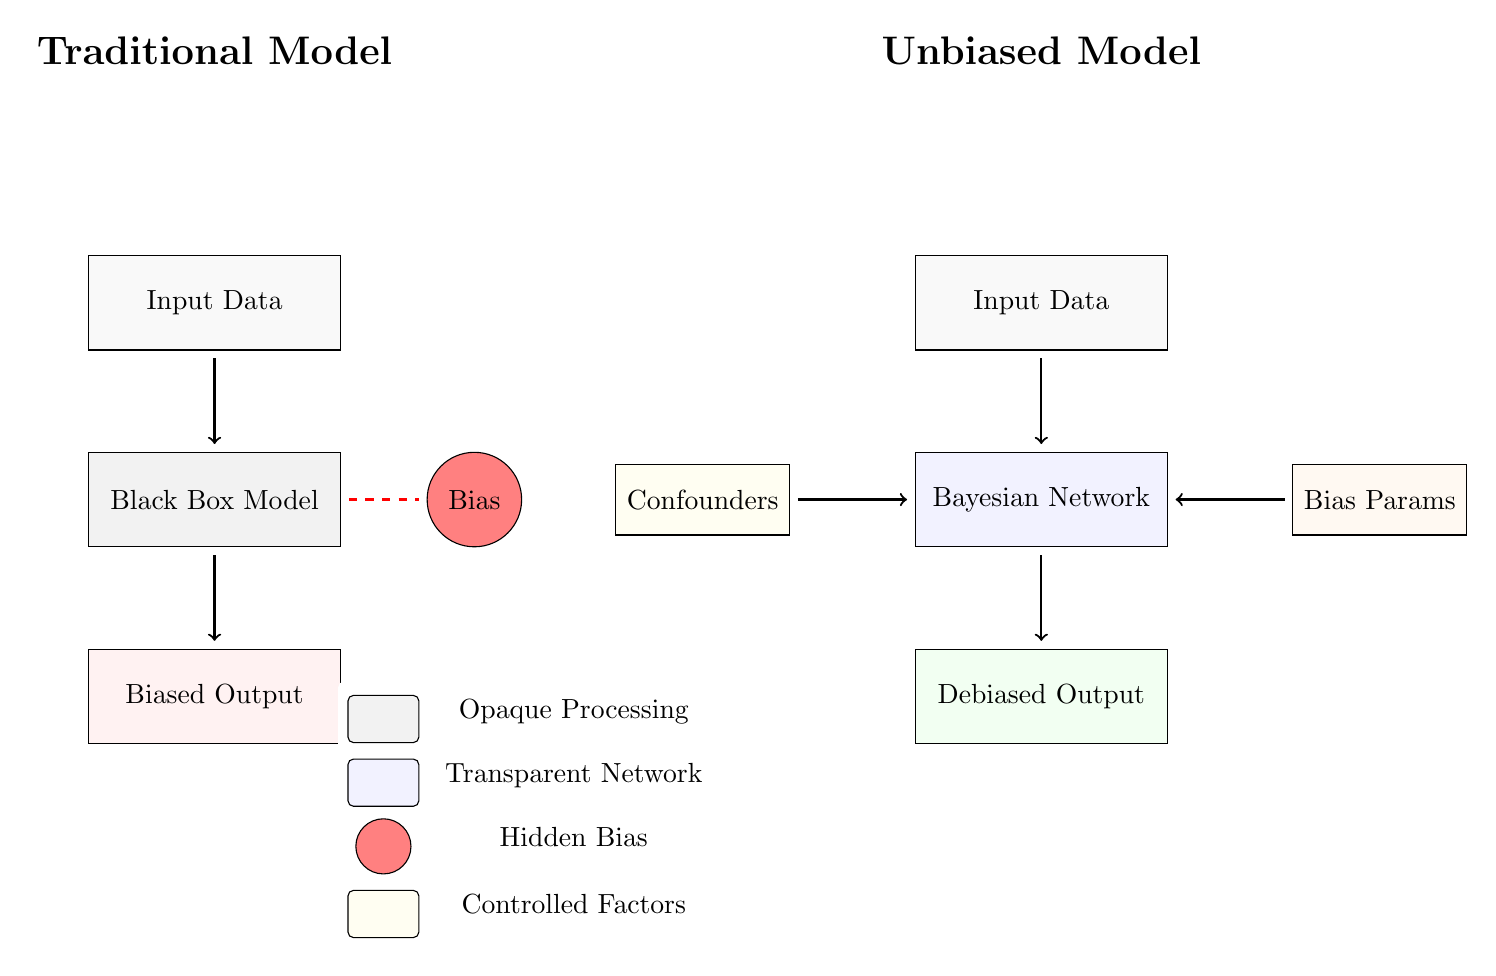
\begin{tikzpicture}[node distance=2.5cm, every node/.style={outer sep=3pt}]
    % Traditional Model (Left) with box model
    \node[draw, rectangle, minimum width=3.2cm, minimum height=1.2cm, 
          inner sep=5pt, fill=gray!5] (input1) {Input Data};
    \node[draw, rectangle, minimum width=3.2cm, minimum height=1.2cm, 
          below of=input1, inner sep=5pt, fill=black!5] (black1) {Black Box Model};
    \node[draw, rectangle, minimum width=3.2cm, minimum height=1.2cm, 
          below of=black1, inner sep=5pt, fill=red!5] (output1) {Biased Output};
    
    % Arrows for traditional model with spacing
    \draw[->, thick] (input1) -- (black1);
    \draw[->, thick] (black1) -- (output1);
    
    % Hidden bias indicator with proper spacing
    \node[draw, circle, fill=red!50, minimum size=1.2cm, right of=black1, 
          xshift=0.8cm, inner sep=2pt] (bias1) {Bias};
    \draw[dashed, red, thick] (black1) -- (bias1);
    
    % Unbiased Model (Right) with box model
    \node[draw, rectangle, minimum width=3.2cm, minimum height=1.2cm, 
          right of=input1, xshift=8cm, inner sep=5pt, fill=gray!5] (input2) {Input Data};
    \node[draw, rectangle, minimum width=3.2cm, minimum height=1.2cm, 
          below of=input2, inner sep=5pt, fill=blue!5] (bayes2) {Bayesian Network};
    \node[draw, rectangle, minimum width=1.8cm, minimum height=0.9cm, 
          left of=bayes2, xshift=-1.8cm, inner sep=4pt, fill=yellow!5] (confound2) {Confounders};
    \node[draw, rectangle, minimum width=1.8cm, minimum height=0.9cm, 
          right of=bayes2, xshift=1.8cm, inner sep=4pt, fill=orange!5] (bias_param2) {Bias Params};
    \node[draw, rectangle, minimum width=3.2cm, minimum height=1.2cm, 
          below of=bayes2, inner sep=5pt, fill=green!5] (output2) {Debiased Output};
    
    % Arrows for unbiased model with spacing
    \draw[->, thick] (input2) -- (bayes2);
    \draw[->, thick] (confound2) -- (bayes2);
    \draw[->, thick] (bias_param2) -- (bayes2);
    \draw[->, thick] (bayes2) -- (output2);
    
    % Labels with proper spacing
    \node[above of=input1, yshift=0.7cm, font=\bfseries] {\Large Traditional Model};
    \node[above of=input2, yshift=0.7cm, font=\bfseries] {\Large Unbiased Model};
    
    % Color-coded key
    \matrix[matrix of nodes, fill=white!90, rounded corners=2pt,
            column sep=6pt, row sep=4pt, ampersand replacement=\&] at (4,-6.5) {
        |[rectangle, draw, fill=black!5, minimum width=0.9cm, minimum height=0.6cm]|  \& Opaque Processing \\
        |[rectangle, draw, fill=blue!5,  minimum width=0.9cm, minimum height=0.6cm]|  \& Transparent Network \\
        |[circle,    draw, fill=red!50,  minimum width=0.7cm, minimum height=0.7cm]|  \& Hidden Bias \\
        |[rectangle, draw, fill=yellow!5,minimum width=0.9cm, minimum height=0.6cm]|  \& Controlled Factors \\
    };
\end{tikzpicture}}
\caption{Architectural Comparison: Traditional vs. Unbiased Model}
\end{figure}

\section{Hypothesis I: AI Bias as Pattern Learning}

\begin{figure}[H]
\centering
\resizebox{0.95\textwidth}{!}{%
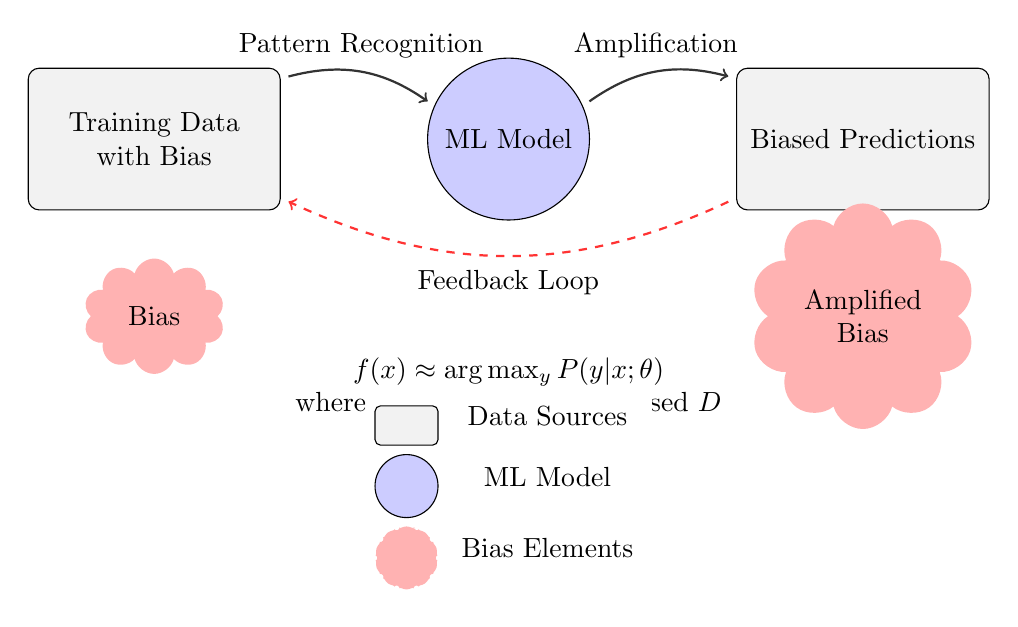
\begin{tikzpicture}[scale=0.9, every node/.style={outer sep=3pt}]
    % Pattern Learning Process with box model spacing
    \node[draw, rectangle, rounded corners, minimum width=3.2cm, minimum height=1.8cm, 
          inner sep=5pt, fill=gray!10, align=center] (data) at (0,0) {Training Data \\ with Bias};
    
    \node[draw, circle, minimum size=1.8cm, inner sep=5pt, fill=blue!20] (model) at (5,0) {ML Model};
    
    \node[draw, rectangle, rounded corners, minimum width=3.2cm, minimum height=1.8cm,
          inner sep=5pt, fill=gray!10] (output) at (10,0) {Biased Predictions};
    
    % Pattern flow with improved spacing
    \draw[->, thick, draw=black!80] (data) to[bend left=25] 
          node[above, inner sep=2pt] {Pattern Recognition} (model);
    \draw[->, thick, draw=black!80] (model) to[bend left=25] 
          node[above, inner sep=2pt] {Amplification} (output);
    \draw[->, thick, dashed, draw=red!80] (output) to[bend left=25] 
          node[below, inner sep=2pt] {Feedback Loop} (data);
    
    % Bias indicators with proper spacing
    \node[fill=red!30, cloud, cloud puffs=10, minimum width=1.8cm, minimum height=1.2cm,
          inner sep=3pt] at (0,-2.5) {Bias};
    \node[fill=red!30, cloud, cloud puffs=10, minimum width=1.8cm, minimum height=1.2cm,
          inner sep=3pt, align=center] at (10,-2.5) {Amplified\\Bias};
    
    % Mathematical representation with spacing
    \node[inner sep=5pt, align=center] at (5,-3.5) {
        $f(x) \approx \arg\max_y P(y|x;\theta)$ \\
        where $\theta$ is optimized over biased $D$
    };
    
    % Color-coded key
    \matrix[matrix of nodes, fill=white!90, rounded corners=2pt,
            column sep=5pt, row sep=3pt, ampersand replacement=\&] at (5,-5) {
        |[rectangle, draw, fill=gray!10, minimum width=0.8cm, minimum height=0.5cm]| {} \& Data Sources \\
        |[circle, draw, fill=blue!20, minimum width=0.8cm, minimum height=0.8cm]| {} \& ML Model \\
        |[cloud, cloud puffs=10, fill=red!30, minimum width=0.8cm, minimum height=0.8cm]| {} \& Bias Elements \\
    };
\end{tikzpicture}}
\caption{Pattern Learning and Bias Amplification}
\end{figure}

\subsection{Hypothesis I Algorithm: Pattern Detection and Amplification}

\begin{algorithm}[H]
\caption{Biased Pattern Learning}
\begin{algorithmic}[1]
    \STATE \textbf{Input:} Dataset $D$ with bias $\phi$
    \STATE \textbf{Output:} ML Model $f$ with amplified bias
    \STATE Initialize model parameters $\theta$
    \FOR{each training epoch}
        \FOR{each sample $(x, y) \in D$}
            \STATE Compute prediction $\hat{y} = f(x; \theta)$
            \STATE Calculate loss $\mathcal{L}(f(x), y)$
            \STATE Update $\theta$ to minimize $\mathcal{L}$
        \ENDFOR
    \ENDFOR
    \STATE \textbf{Result:} Model replicates biased patterns
\end{algorithmic}
\end{algorithm}

\section{Hypothesis II: Unboxing Through Data Structure Awareness}

\begin{figure}[H]
\centering
\resizebox{0.95\textwidth}{!}{%
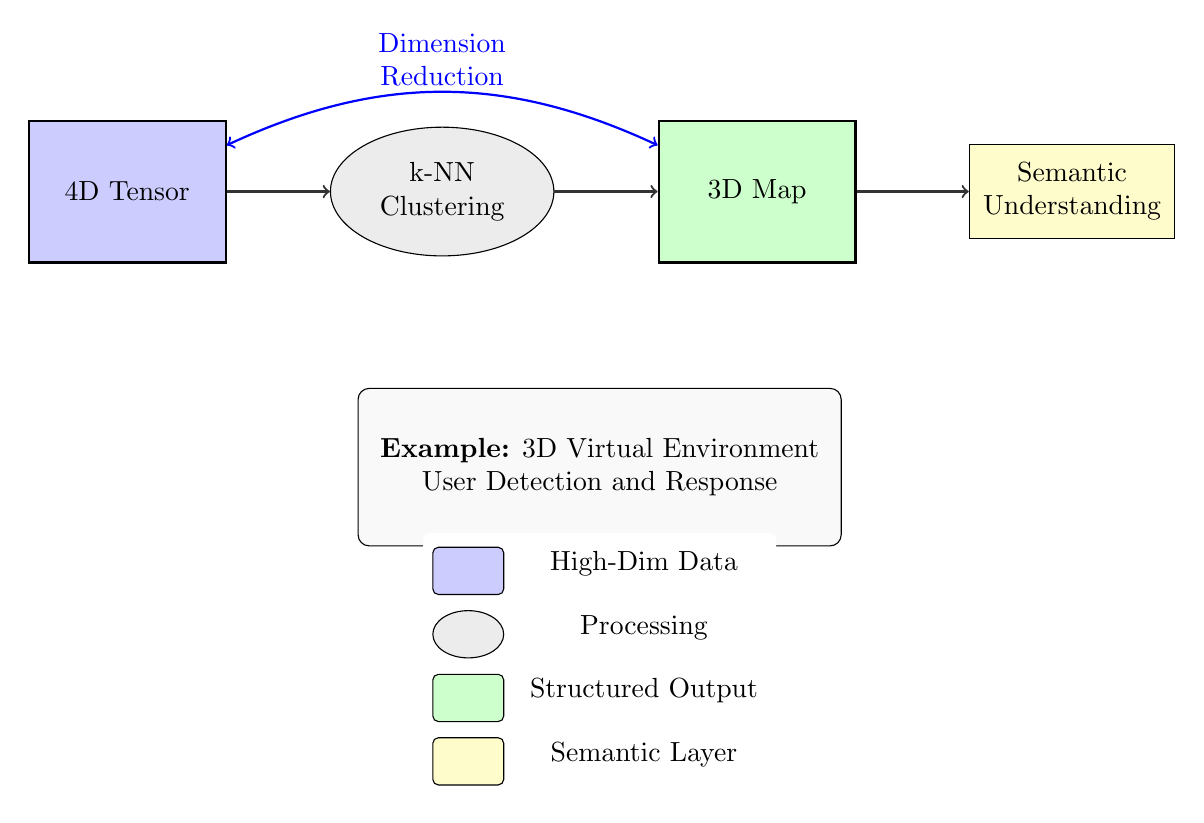
\begin{tikzpicture}[
    data block/.style={rectangle, draw, minimum width=2cm, minimum height=1.2cm, inner sep=5pt},
    tensor/.style={rectangle, draw, thick, minimum width=2.5cm, minimum height=1.8cm, inner sep=6pt},
    process/.style={ellipse, draw, minimum width=2.5cm, minimum height=1.2cm, inner sep=6pt}
]
    % 4D to 3D transformation with proper spacing
    \node[tensor, fill=blue!20] (tensor4d) at (0,0) {4D Tensor};
    \node[process, fill=gray!15, align=center] (cluster) at (4,0) {k-NN\\Clustering};
    \node[tensor, fill=green!20] (tensor3d) at (8,0) {3D Map};
    \node[data block, fill=yellow!20, align=center] (semantic) at (12,0) {Semantic\\Understanding};
    
    % Flow arrows with spacing
    \draw[->, thick, draw=black!80] (tensor4d) -- (cluster);
    \draw[->, thick, draw=black!80] (cluster) -- (tensor3d);
    \draw[->, thick, draw=black!80] (tensor3d) -- (semantic);
    
    % Example scenario with box model
    \node[draw, rounded corners, minimum width=5cm, minimum height=2cm, 
          inner sep=8pt, fill=gray!5, align=center] at (6,-3.5) {
        \textbf{Example:} 3D Virtual Environment\\
        User Detection and Response
    };
    
    % Dimensional reduction with proper spacing
    \draw[<->, thick, blue] (tensor4d) to[bend left=25] 
          node[above, sloped, align=center, inner sep=2pt] {Dimension\\Reduction} (tensor3d);
    
    % Color-coded key
    \matrix[matrix of nodes, fill=white!90, rounded corners=2pt,
            column sep=6pt, row sep=4pt, ampersand replacement=\&] at (6,-6) {
        |[rectangle, draw, fill=blue!20, minimum width=0.9cm, minimum height=0.6cm]| {} \& High-Dim Data \\
        |[ellipse, draw, fill=gray!15, minimum width=0.9cm, minimum height=0.6cm]| {} \& Processing \\
        |[rectangle, draw, fill=green!20, minimum width=0.9cm, minimum height=0.6cm]| {} \& Structured Output \\
        |[rectangle, draw, fill=yellow!20, minimum width=0.9cm, minimum height=0.6cm]| {} \& Semantic Layer \\
    };
\end{tikzpicture}}
\caption{Data Structure Unboxing Process}
\end{figure}

\subsection{Hypothesis II Algorithm: Structural Unboxing}

\begin{algorithm}[H]
\caption{Data Structure Unboxing}
\begin{algorithmic}[1]
    \STATE \textbf{Input:} 4D tensor data $T_{4D}$
    \STATE \textbf{Output:} Semantically structured map
    \STATE Apply k-NN clustering on $T_{4D}$
    \STATE Group data by similarity metrics
    \STATE Transform to 3D representation
    \STATE Ungroup for semantic map creation
    \STATE Match structure to problem domain
    \RETURN Structured semantic map
\end{algorithmic}
\end{algorithm}

\section{Hypothesis III: Modular System Architecture}

\begin{figure}[H]
\centering
\resizebox{0.9\textwidth}{!}{%
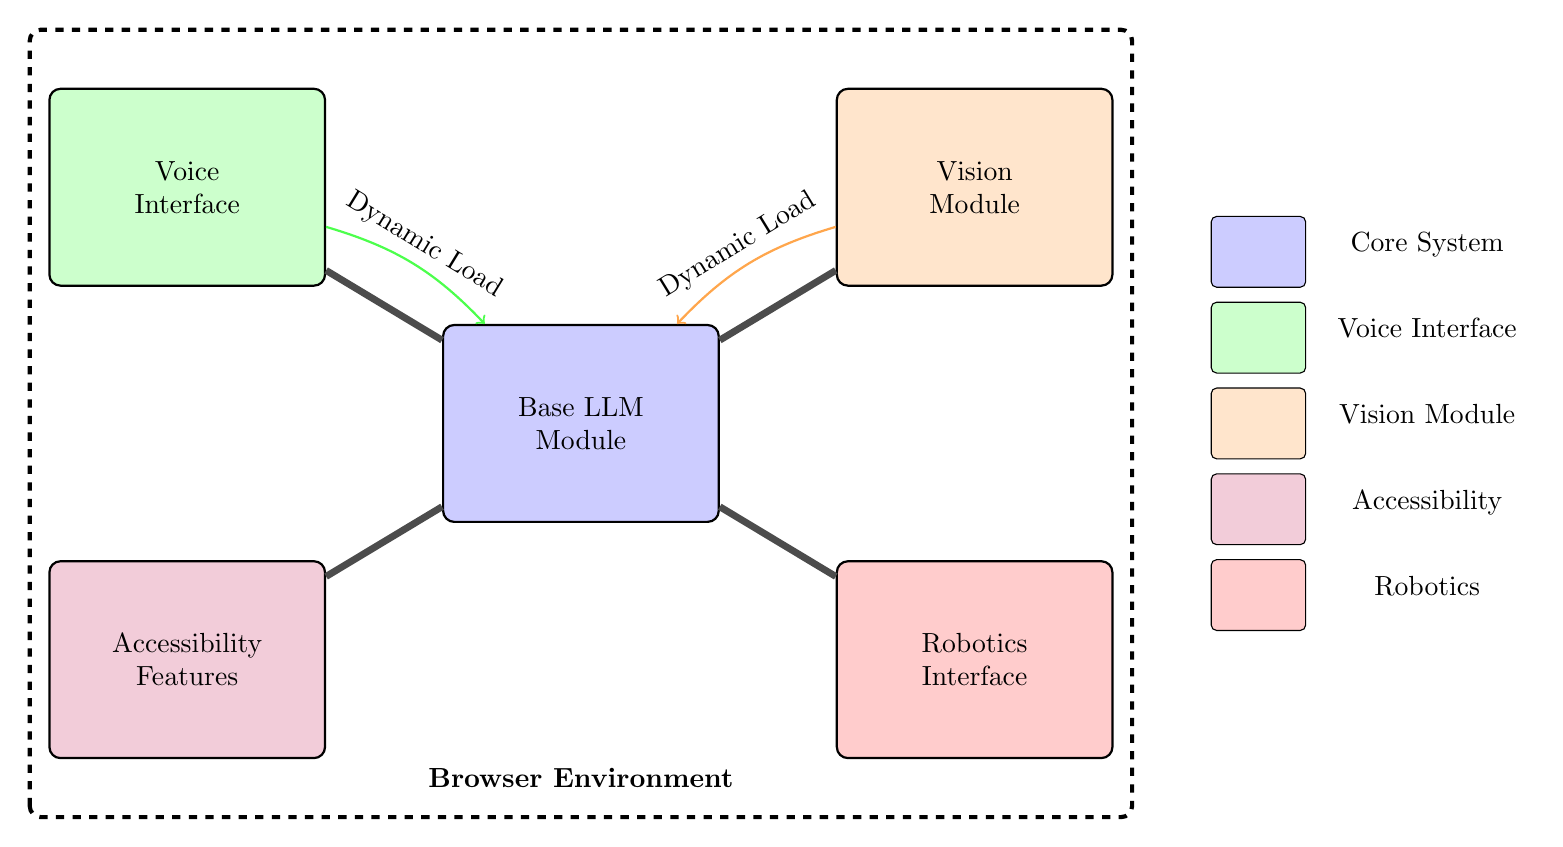
\begin{tikzpicture}[
    module/.style={rectangle, draw, thick, minimum width=3.5cm, minimum height=2.5cm, align=center,
                   rounded corners, inner sep=8pt},
    connector/.style={line width=2.5pt, draw=black!70}
]
    % Core LLM Module with box model spacing
    \node[module, fill=blue!20] (llm) at (0,0) {Base LLM\\Module};
    
    % Surrounding modules with proper spacing
    \node[module, fill=green!20] (voice) at (-5,3) {Voice\\Interface};
    \node[module, fill=orange!20] (vision) at (5,3) {Vision\\Module};
    \node[module, fill=purple!20] (access) at (-5,-3) {Accessibility\\Features};
    \node[module, fill=red!20] (robotics) at (5,-3) {Robotics\\Interface};
    
    % Browser container with padding
    \draw[dashed, thick, rounded corners, line width=1.5pt] 
         (-7,-5) rectangle (7,5);
    \node[inner sep=4pt] at (0,-4.5) {\textbf{Browser Environment}};
    
    % Connections with visual separation
    \draw[connector] (llm) -- (voice);
    \draw[connector] (llm) -- (vision);
    \draw[connector] (llm) -- (access);
    \draw[connector] (llm) -- (robotics);
    
    % Dynamic loading arrows with better spacing
    \draw[->, bend left=15, thick, draw=green!70] (voice) to 
          node[above, sloped, inner sep=3pt] {Dynamic Load} (llm);
    \draw[->, bend right=15, thick, draw=orange!70] (vision) to 
          node[above, sloped, inner sep=3pt] {Dynamic Load} (llm);
    
    % Color-coded key
    \matrix[matrix of nodes, fill=white!90, rounded corners=2pt, column sep=8pt, row sep=5pt,
            ampersand replacement=\&] at (10,0) {
        |[rectangle, draw, fill=blue!20, minimum width=1.2cm, minimum height=0.9cm]| {} \& Core System \\
        |[rectangle, draw, fill=green!20, minimum width=1.2cm, minimum height=0.9cm]| {} \& Voice Interface \\
        |[rectangle, draw, fill=orange!20, minimum width=1.2cm, minimum height=0.9cm]| {} \& Vision Module \\
        |[rectangle, draw, fill=purple!20, minimum width=1.2cm, minimum height=0.9cm]| {} \& Accessibility \\
        |[rectangle, draw, fill=red!20, minimum width=1.2cm, minimum height=0.9cm]| {} \& Robotics \\
    };
\end{tikzpicture}}
\caption{Modular AI System Architecture}
\end{figure}

\subsection{Hypothesis III Algorithm: Modular Component Loading}

\begin{algorithm}[H]
\caption{Dynamic Module Loading}
\begin{algorithmic}[1]
    \STATE \textbf{Input:} Module requirements
    \STATE Initialize core LLM module
    \FOR{each required feature}
        \STATE Identify module from directory tree
        \STATE Load module dynamically
        \STATE Connect to core system
        \STATE Validate integration
    \ENDFOR
    \STATE Optimize performance based on loaded modules
    \RETURN Configured modular system
\end{algorithmic}
\end{algorithm}

\section{Bayesian Network Implementation}

\begin{figure}[H]
\centering
\resizebox{0.9\textwidth}{!}{%
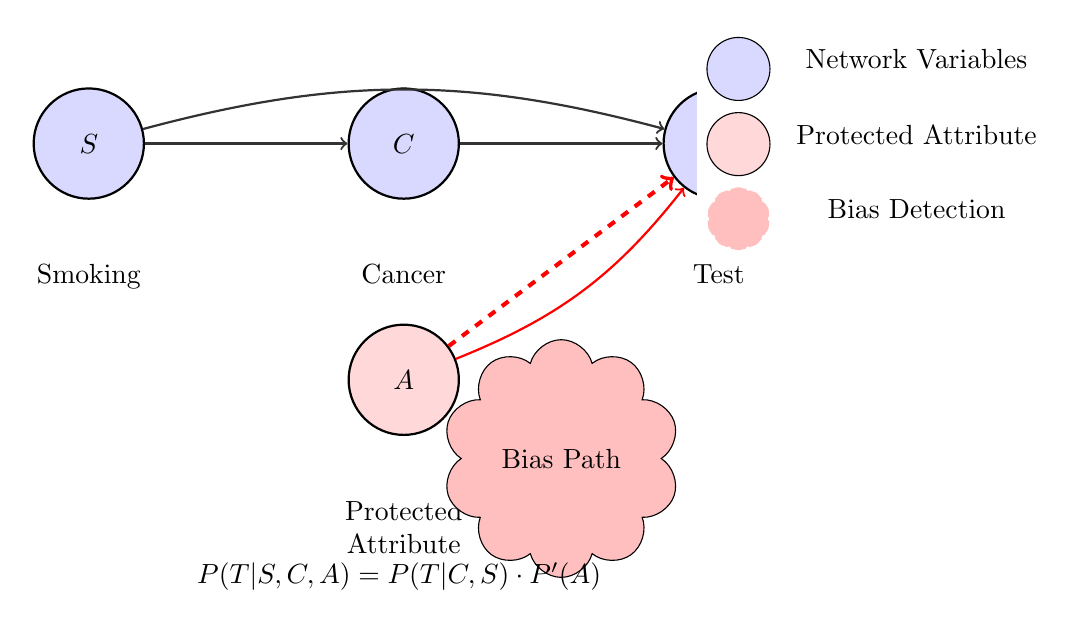
\begin{tikzpicture}[
    node distance=3cm,
    mynode/.style={circle, draw, thick, minimum size=1.4cm, inner sep=4pt},
    direction/.style={->, thick, draw=black!80}
]
    % Variables with proper spacing
    \node[mynode, fill=blue!15] (S) at (0,0) {$S$};
    \node[mynode, fill=blue!15] (C) at (4,0) {$C$};
    \node[mynode, fill=blue!15] (T) at (8,0) {$T$};
    \node[mynode, fill=red!15] (A) at (4,-3) {$A$};
    
    % Labels with spacing
    \node[below=0.7cm of S, align=center] {Smoking};
    \node[below=0.7cm of C, align=center] {Cancer};
    \node[below=0.7cm of T, align=center] {Test};
    \node[below=0.7cm of A, align=center] {Protected\\Attribute};
    
    % Directed edges with proper visual spacing
    \draw[direction] (S) -- (C);
    \draw[direction] (C) -- (T);
    \draw[direction] (S) to[bend left=15] (T);
    \draw[direction, dashed, red, line width=1.5pt] (A) -- (T);
    
    % Bias path with box model
    \node[draw, cloud, cloud puffs=10, fill=red!25, minimum width=1.8cm, 
          minimum height=1.2cm, inner sep=4pt] at (6,-4) {Bias Path};
    \draw[->, red, thick] (A) to[bend right=15] (T);
    
    % Mathematical formula with proper spacing
    \node[inner sep=8pt, align=center] at (4,-5.5) {
        $P(T|S,C,A) = P(T|C,S) \cdot P'(A)$
    };
    
    % Color-coded key
    \matrix[matrix of nodes, fill=white!90, rounded corners=2pt,
            column sep=6pt, row sep=4pt, ampersand replacement=\&] at (10,0) {
        |[circle, draw, fill=blue!15, minimum width=0.8cm, minimum height=0.8cm]| {} \& Network Variables \\
        |[circle, draw, fill=red!15, minimum width=0.8cm, minimum height=0.8cm]| {} \& Protected Attribute \\
        |[cloud, cloud puffs=10, fill=red!25, minimum width=0.8cm, minimum height=0.8cm]| {} \& Bias Detection \\
    };
\end{tikzpicture}}
\caption{Bayesian Network with Bias Detection}
\end{figure}

\section{Formal Proof Framework}

\subsection{Traditional vs. Bayesian Inference}

\begin{align}
\text{Traditional:} \quad \theta^* &= \arg\max_\theta P(\theta|D) \approx \text{biased optimum}\\
\text{Bayesian:} \quad P(\theta|D) &= \int P(\theta,\phi|D)d\phi
\end{align}

\begin{figure}[H]
\centering
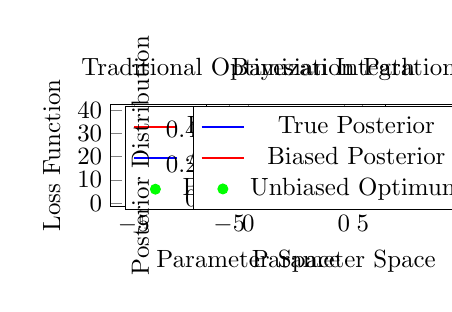
\begin{tikzpicture}[scale=0.9]
    % Traditional approach visualization
    \begin{axis}[
        title={Traditional Optimization Path},
        xlabel={Parameter Space},
        ylabel={Loss Function},
        width=0.45\textwidth,
        height=0.25\textwidth,
        domain=-5:5,
        samples=100
    ]
        \addplot[color=red, thick] {x^2 - 2*x + 3};
        \addplot[color=blue, thick] {x^2 - 2*x + 4};
        \addplot[color=green, mark=*, only marks] coordinates {(1,2)};
        \addlegendentry{Biased Function}
        \addlegendentry{Actual Function}
        \addlegendentry{Biased Optimum}
    \end{axis}
    
    % Bayesian approach visualization
    \hspace{0.1\textwidth}
    \begin{axis}[
        title={Bayesian Integration},
        xlabel={Parameter Space},
        ylabel={Posterior Distribution},
        width=0.45\textwidth,
        height=0.25\textwidth,
        domain=-5:5,
        samples=100
    ]
        \addplot[color=blue, thick, fill=blue!20] {exp(-(x-1)^2/2)/sqrt(2*pi)};
        \addplot[color=red, thick] {exp(-(x-2)^2/4)/2};
        \addplot[color=green, mark=*, only marks] coordinates {(1.5,0.3)};
        \addlegendentry{True Posterior}
        \addlegendentry{Biased Posterior}
        \addlegendentry{Unbiased Optimum}
    \end{axis}
\end{tikzpicture}
\caption{Optimization Comparison: Traditional vs. Bayesian}
\end{figure}

\section{Implementation Roadmap}

\begin{figure}[H]
\centering
\resizebox{0.95\textwidth}{!}{%
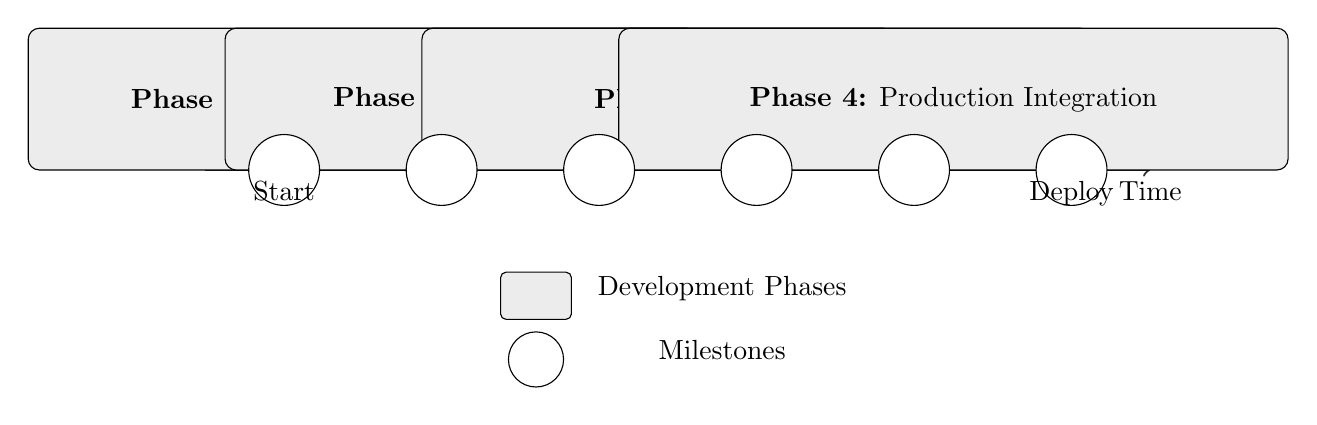
\begin{tikzpicture}[
    phase/.style={rectangle, draw, rounded corners, minimum width=8.5cm, minimum height=1.8cm,
                  fill=gray!15, inner sep=6pt},
    milestone/.style={circle, draw, minimum size=0.9cm, fill=white, inner sep=1pt}
]
    % Timeline with proper spacing
    \draw[->, thick, draw=black!80] (0,0) -- (12,0);
    \node[below, inner sep=4pt] at (12,0) {Time};
    
    % Phases with box model spacing
    \node[phase] at (2,0.9) {\textbf{Phase 1:} Mathematical Formulations};
    \node[phase] at (4.5,0.9) {\textbf{Phase 2:} Algorithm Implementation};
    \node[phase] at (7,0.9) {\textbf{Phase 3:} Validation Suite};
    \node[phase] at (9.5,0.9) {\textbf{Phase 4:} Production Integration};
    
    % Milestones with spacing
    \foreach \x in {1,3,5,7,9,11} {
        \node[milestone] at (\x,0) {};
    }
    
    % Labels with proper spacing
    \node[below, inner sep=4pt] at (1,0) {Start};
    \node[below, inner sep=4pt] at (11,0) {Deploy};
    
    % Color-coded key
    \matrix[matrix of nodes, fill=white!90, rounded corners=2pt,
            column sep=6pt, row sep=4pt, ampersand replacement=\&] at (6,-2) {
        |[rectangle, draw, fill=gray!15, minimum width=0.9cm, minimum height=0.6cm]| {} \& Development Phases \\
        |[circle, draw, fill=white, minimum width=0.7cm, minimum height=0.7cm]| {} \& Milestones \\
    };
\end{tikzpicture}}
\caption{Development Roadmap}
\end{figure}

\section{Expected Outcomes}

\begin{table}[H]
\centering
\begin{tabular}{|l|c|c|}
\hline
\textbf{Metric} & \textbf{Traditional} & \textbf{Bayesian} \\
\hline
Demographic Fairness & Low & High \\
Transparency & None & Complete \\
Uncertainty Quantification & None & Explicit \\
Performance Disparity & High & Reduced \\
Regulatory Compliance & Difficult & Auditable \\
\hline
\end{tabular}
\caption{Performance Comparison}
\end{table}

\section{Conclusion}

This framework establishes a formal mathematical foundation for addressing bias in AI systems through Bayesian modeling. By combining theoretical rigor with practical implementation strategies, we create more equitable and transparent machine learning systems that can be verified and audited.

\subsection{Key Contributions}
\begin{itemize}
    \item Formal proof of bias emergence in pattern-based learning
    \item Structural unboxing methodology for data awareness
    \item Modular architecture for scalable AI systems
    \item Bayesian framework for explicit bias mitigation
\end{itemize}

\begin{thebibliography}{9}
\bibitem{pearl2000}
Pearl, J. (2000). Causality: Models, Reasoning, and Inference. Cambridge University Press.

\bibitem{goodfellow2016}
Goodfellow, I., Bengio, Y., Shlens, J. (2016). Explaining and Harnessing Adversarial Examples. ICLR 2016.

\bibitem{barocas2016}
Barocas, S., Hardt, M., Narayanan, A. (2019). Fairness and Machine Learning. fairmlbook.org

\bibitem{gelman2013}
Gelman, A., et al. (2013). Bayesian Data Analysis. Chapman \& Hall/CRC.
\end{thebibliography}

\appendix

\section{Mathematical Derivations}

For the marginal posterior computation:
\begin{align}
P(\theta|D) &= \int P(\theta,\phi|D)d\phi\\
&= \int \frac{P(D|\theta,\phi)P(\theta,\phi)}{P(D)}d\phi\\
&= \frac{1}{P(D)}\int P(D|\theta,\phi)P(\theta|\phi)P(\phi)d\phi
\end{align}

\section{Implementation Notes}

\begin{itemize}
    \item Use INLA or Stan for efficient Bayesian computation
    \item Implement parallel processing for 4D tensor operations
    \item Create modular APIs for dynamic component loading
    \item Design thorough testing suites for bias metrics
\end{itemize}

\end{document}